\documentclass[paper=letter,11pt]{scrartcl}

\KOMAoptions{headinclude=true, footinclude=false}
\KOMAoptions{DIV=14, BCOR=5mm}
\KOMAoptions{numbers=noendperiod}
\KOMAoptions{parskip=half}
\addtokomafont{disposition}{\rmfamily}
\addtokomafont{part}{\LARGE}
\addtokomafont{descriptionlabel}{\rmfamily}
%\setkomafont{pageheadfoot}{\normalsize\sffamily}
\setkomafont{pagehead}{\normalsize\rmfamily}
%\setkomafont{publishers}{\normalsize\rmfamily}
\setkomafont{caption}{\normalfont\small}
\setcapindent{0pt}
\deffootnote[1em]{1em}{1em}{\textsuperscript{\thefootnotemark}\ }


\usepackage{amsmath}
\usepackage[varg]{txfonts}
\usepackage[T1]{fontenc}
\usepackage{graphicx}
\usepackage{xcolor}
\usepackage[american]{babel}
% hyperref is needed in many places, so include it here
\usepackage{hyperref}

\usepackage{xspace}
\usepackage{multirow}
\usepackage{float}


\usepackage{braket}
\usepackage{bbm}
\usepackage{relsize}
\usepackage{tcolorbox}

\def\ketY{\ensuremath{\ket {\Psi}}}
\def\iGeV{\ensuremath{\textrm{GeV}^{-1}}}
%\def\mp{\ensuremath{m_{\textrm{proton}}}}
\def\rp{\ensuremath{r_{\textrm{proton}}}}
\def\me{\ensuremath{m_{\textrm{electron}}}}
\def\aG{\ensuremath{\alpha_G}}
\def\rAtom{\ensuremath{r_{\textrm{atom}}}}
\def\rNucl{\ensuremath{r_{\textrm{nucleus}}}}
\def\GN{\ensuremath{\textrm{G}_\textrm{N}}}
\def\ketX{\ensuremath{\ket{\vec{x}}}}
\def\ve{\ensuremath{\vec{\epsilon}}}


\def\ABCDMatrix{\ensuremath{\begin{pmatrix} A &  B  \\ C  & D \end{pmatrix}}}
\def\xyprime{\ensuremath{\begin{pmatrix} x' \\ y' \end{pmatrix}}}
\def\xyprimeT{\ensuremath{\begin{pmatrix} x' &  y' \end{pmatrix}}}
\def\xy{\ensuremath{\begin{pmatrix} x \\ y \end{pmatrix}}}
\def\xyT{\ensuremath{\begin{pmatrix} x & y \end{pmatrix}}}

\def\IMatrix{\ensuremath{\begin{pmatrix} 0 &  1  \\ -1  & 0 \end{pmatrix}}}
\def\IBoostMatrix{\ensuremath{\begin{pmatrix} 0 &  1  \\ 1  & 0 \end{pmatrix}}}
\def\JThree{\ensuremath{\begin{pmatrix}    0 & -i & 0  \\ i & 0  & 0 \\ 0 & 0 & 0 \end{pmatrix}}} 
\def\JTwo{\ensuremath{\begin{bmatrix}    0 & 0 & -i  \\ 0 & 0  & 0 \\ i & 0 & 0 \end{bmatrix}}}
\def\JOne{\ensuremath{\begin{bmatrix}    0 & 0 & 0  \\ 0 & 0  & -i \\ 0 & i & 0 \end{bmatrix}}}
\def\etamn{\ensuremath{\eta_{\mu\nu}}}
\def\Lmn{\ensuremath{\Lambda^\mu_\nu}}
\def\dmn{\ensuremath{\delta^\mu_\nu}}
\def\wmn{\ensuremath{\omega^\mu_\nu}}
\def\be{\begin{equation*}}
\def\ee{\end{equation*}}
\def\bea{\begin{eqnarray*}}
\def\eea{\end{eqnarray*}}
\def\bi{\begin{itemize}}
\def\ei{\end{itemize}}
\def\fmn{\ensuremath{F_{\mu\nu}}}
\def\fMN{\ensuremath{F^{\mu\nu}}}
\def\bc{\begin{center}}
\def\ec{\end{center}}
\def\nus{$\nu$s}

\def\adagger{\ensuremath{a_{p\sigma}^\dagger}}
\def\lineacross{\noindent\rule{\textwidth}{1pt}}

\newcommand{\multiline}[1] {
\begin{tabular} {|l}
#1
\end{tabular}
}

\newcommand{\multilineNoLine}[1] {
\begin{tabular} {l}
#1
\end{tabular}
}



\newcommand{\lineTwo}[2] {
\begin{tabular} {|l}
#1 \\
#2
\end{tabular}
}

\newcommand{\rmt}[1] {
\textrm{#1}
}


%
% Units
%
\def\m{\ensuremath{\rmt{m}}}
\def\GeV{\ensuremath{\rmt{GeV}}}
\def\pt{\ensuremath{p_\rmt{T}}}


\def\parity{\ensuremath{\mathcal{P}}}

\usepackage{cancel}
\usepackage{ mathrsfs }
\def\bigL{\ensuremath{\mathscr{L}}}

\usepackage{ dsfont }



\usepackage{fancyhdr}
\fancyhf{}

%\documentclass[margin,line]{res}
\usepackage{braket}
\usepackage{bbm}
\usepackage{relsize}

\def\ketY{\ensuremath{\ket {\Psi}}}
\def\iGeV{\ensuremath{\textrm{GeV}^{-1}}}


\def\ABCDMatrix{\ensuremath{\begin{pmatrix} A &  B  \\ C  & D \end{pmatrix}}}
\def\xyprime{\ensuremath{\begin{pmatrix} x' \\ y' \end{pmatrix}}}
\def\xyprimeT{\ensuremath{\begin{pmatrix} x' &  y' \end{pmatrix}}}
\def\xy{\ensuremath{\begin{pmatrix} x \\ y \end{pmatrix}}}
\def\xyT{\ensuremath{\begin{pmatrix} x & y \end{pmatrix}}}

\def\IMatrix{\ensuremath{\begin{pmatrix} 0 &  1  \\ -1  & 0 \end{pmatrix}}}
\def\IBoostMatrix{\ensuremath{\begin{pmatrix} 0 &  1  \\ 1  & 0 \end{pmatrix}}}
\def\JThree{\ensuremath{\begin{pmatrix}    0 & -i & 0  \\ i & 0  & 0 \\ 0 & 0 & 0 \end{pmatrix}}} 
\def\JTwo{\ensuremath{\begin{bmatrix}    0 & 0 & -i  \\ 0 & 0  & 0 \\ i & 0 & 0 \end{bmatrix}}}
\def\JOne{\ensuremath{\begin{bmatrix}    0 & 0 & 0  \\ 0 & 0  & -i \\ 0 & i & 0 \end{bmatrix}}}
\def\etamn{\ensuremath{\eta_{\mu\nu}}}
\def\Lmn{\ensuremath{\Lambda^\mu_\nu}}
\def\dmn{\ensuremath{\delta^\mu_\nu}}
\def\wmn{\ensuremath{\omega^\mu_\nu}}
\def\be{\begin{equation*}}
\def\ee{\end{equation*}}
\def\bc{\begin{center}}
\def\ec{\end{center}}
\def\nus{$\nu$s}
%\def\xMu{\ensuremath{x^\mu}

\usepackage{fancyhdr}

\fancyhf{}
\lhead{\Large 33-444} % \hfill Introduction to Particle Physics \hfill Spring 2019}
\chead{\Large Introduction to Particle Physics} % \hfill Spring 2019}
\rhead{\Large Spring 2019} % \hfill Introduction to Particle Physics \hfill Spring 2019}

\begin{document}
\thispagestyle{fancy}

\begin{center}
{\huge \textbf{Lecture 34}}
\end{center}

{\fontsize{14}{16}\selectfont

\textbf{\underline{Neutrino Physics}} 

\underline{Bottom line}: Solar fusion takes lighter nuclei and might bigger ones.
Also important to know is that the sun is very proton rich, not many neutrons (lots of electrons), so in the process of forming nuclei can convince yourself that you also emit a lot of \nus. 
not anti-\nus, proper \nus.   
This is the opposite of $\beta$ decay. 

$\beta$ decay is usually from nuclei that have too many neutrons in them. 
So they are happy to convert into protons and emit anti-neutrinos at the same time. 
On the flip side if you have an environment that is proton-rich and you are creating nuclei that mean you are converting protons into neutrons to balance out the charge you have to spit out positrons and neutrons to conserve lepton number. 
The sun is very efficient machine for producing neutrinos. 

When people finally figured out how the sun worked they said ``hey look the sun is spitting out all these \nus wouldn't it be great if we could see them.''
People started thinking about how to do this. 

We can calculate the flux of neutrinos coming from the sun,  its a very high number. $10^{11}/s/cm^2$ on earth. 
And we can calculate what energies they have.  
Here's what you get:

\begin{figure}[h!]
\centering
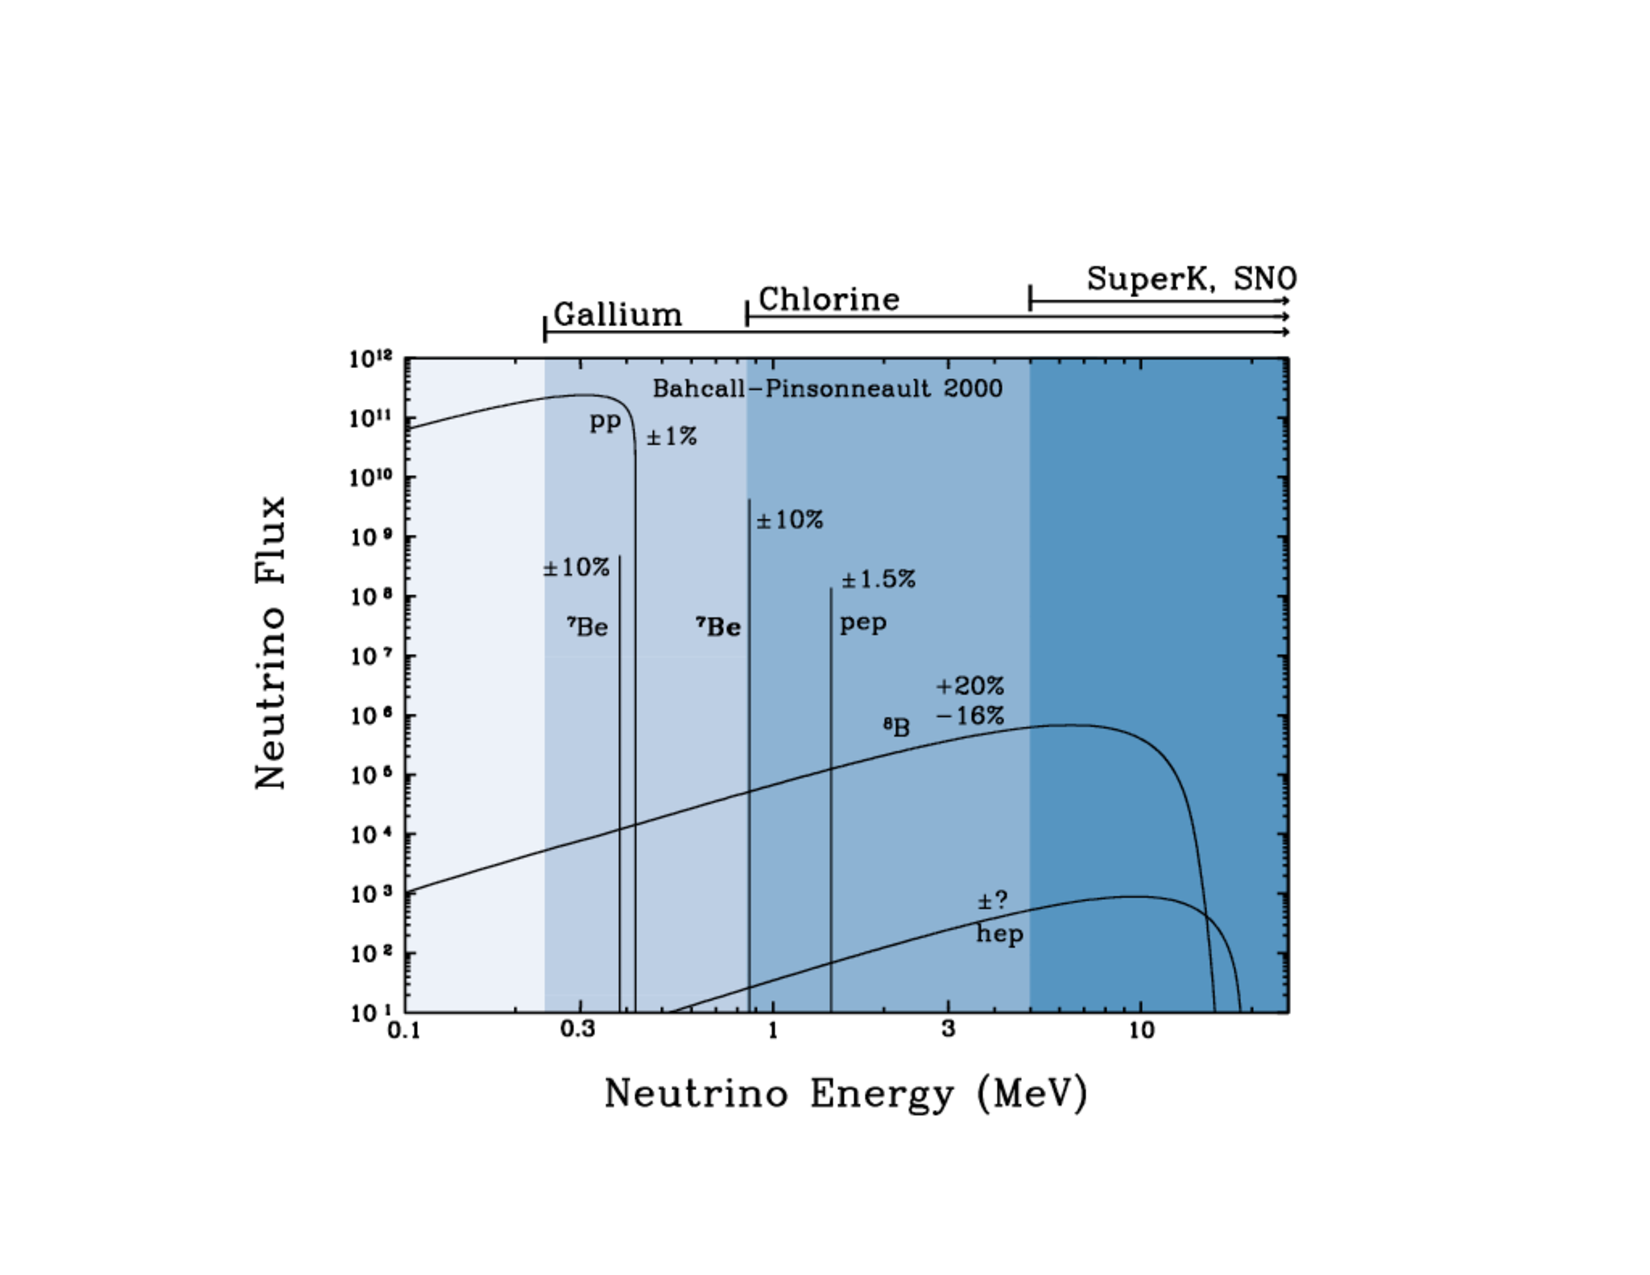
\includegraphics[width=1.0\textwidth]{./NuFromSun.pdf}
\end{figure}

Will pick up here next time...

Turns out the \nus are relatively low energy (below 10 MeV) ``low energy \nus''
How do we detect? these \nus ?
Weve developed 

The oldes one was an experiment that started in the 60s using chorine. 
How do you detewct these very low energy \nus ?
Remember cross sections are very small.
So you need a large amount of something that is going to be your tartget. 
Now you would like to them see them by having them hit someing, only interact via W or Z. 
If interact via Z at these really low energies the best you can get is that if the $\nu$ hits something it will make that something recol. 
(This turns out is actually a problem for DM experiments, but we will come back to this later) 
Very challenging to observe.  
$\nu$ comes in and it hits something and a necleous recoils a little bit. 
We have just observed this about a year ago. (Ironic that this will likely be the biggest backgroudn for DM detection in the future, physics process took so long to measure) 

Other process you can look for is that a $\nu$ hits somehting and it will produce an electron. 
Sort of in busssiness b/c you have an electron, but the big challenge is you live in a big complicated evirements.
And you have to get a signal from a low energy elecgron (b/c the \nus are low eneregy) 
So the ideas that people had for how to measure these \nus in the begingiing were different than standard wasy that particle physiscst would think about doing an experiment. 
First one was a chlorine experiment. 

$\nu + Cl \rightarrow e + Ar$
(If we had a period table we could confirm this) 
And the idea is that you ahve a really big detector made out of clorine and the \nus produce Ar and you are going to see this Ar. 
Great idea b/c Ar is noble gas (wont mix with environment), so if you have a way of separating ar and Cl you're in good shape. 
Actually better than this bc you make the Ar in an excited state that has a fairly long lifetime. 
You can get the AR out and look for Ars decaying, Very cleaver idea. 

Can do the samething with Gallium and Germanium. 

Very very very hard experiments. Just from the shear numebrs that you have to work with. 
Ray Davis experiment. 

Cl is easy to get, buy it in the store (cleaning liquid)
But it a gigantic vat, wait for a month, and the signal is a handful of atome/month in a massive tank of Cl. 
Think tanker truck of cl, looking for a few atoms every month.
Very hard/ very unusual for particle phsyics people/  mostly involves a lot of chemistry (chemistry is very hard) .

Made this measurement for about 40 years. 
Very exicity 
1st of all saw \nus coming from the sun!
Most important for us, saw few \nus that expected, not by a little bit,  say 1/3 of \nus expected. 

Now Historically, most people did not care about this at all.
For several reasons, 
1) doing a really hard experiment, correct to within factor of 3, thats a great result
2) calculations to know what to expect is also very hard 

Things started changing qualitiatively when the very large water detectors starting coming into the game. 
they chose to measure something else, 
For a $\nu$ in water there are three potential targets,  O, H, electrons
Oxygen very unhappy to be hit by \nus and give electron. 

$O \rightarrow N'$
 Oxygen is a very stable nucleus, doesnt like to be turned into other nuclei. 
\nus have a hard time hitting protons/ bc of lepton numebr conservation. 
They woul dhave to produce electrons. proton already has +charge.  Proton would have to turn into somehting with double-plue charge which you cant do at low energies. 
So in the warter detectors the things you can hit are the electrons. 

$\nu + e \rightarrow \nu + e$ (very interesting process) 
Turns out that in these very big water tanks (that were constrcuted to see proton decay) we could see electrons.
even relatively low electrons, can see MeV type electrons. This is crenkov radiation that you read all about on last homework) 
late 80s early 90s

(Should have mentioned this before. 
Clorine detector, first thing they did was put it next ot nuclear reactor, strong sourse of anti-nus 
Curiously enough they didnt see anything, which is actually a big deal, (knew they werent supposed to see anything. reactor emitting anti-nus) 
The clorine reaction doesnt work with anti-nus. 

Side note: 
Interesting they didnt see anything, (this was done in US, rumor that they did see something, perculated to europe and then to soviet union) 
Pontecorvo, who was in exile then came up with a model of hwo a nu can behave like an anti-nu.
model of $\nu$/ $anti-\nu$ oscillations. eventually morphed into the nu oscillations that we know today (among flavours) 


OK so there are the results of these measurements

figure 

These are complicated plots. 
The colored bars  are the expectations for what you should see.
And the blue measurements are how many nus the where actually observed.  
If you ignore the right hand bars for a second.
The rest of teh picture is what is called hte ``solar neutrino puzzle''. 
Seeing few nus that we expected. 
We did a bunch of different experiments.  
So that if you didnt believe the initial Cl expierment, there were all these other experiments that were seeing a deficit. 

Lots of logical possiblities for whats going wrong. 
1) all making a coherent mistake, but this is why we do lots of expirements.  Very unlikely that they all can be going wrong. 
2) our understanding of the sun is not as good as we thought it was.  
    Turns out, for detailed reasons I wont go into, we knew  that the solar model wasnt wrong at the level we needed to explain the data
last hypothsis) or our understanding of how nus propogate is wrong. 

For the last option ther are a lot of things you could think about. 
 -) Maybe \nus decay...
 -) Maybe they get absorbed, 
 -) One hypthesis people raised was the flavoud changing hypethosis

Very simple hypothesis, we will come back to he mechinaism later. 
Basic idea, even if the sun can only produce electron nus, by the time they get here some of them are actuallyinto muon or tau nus. 
That can actually explain all of this.  
All of your experiments are only (mainly) sensitive to electron nus

$\nu_e + e \rightarrow \nu_e + e$  (has both neutral and charged currents) 
$\nu_{\mu,\tau} + e \rightarrow \nu_{\mu,\tau} + e$  (only has neutral currents, only $\sim50\%$ of the cross section ) 


So now we actually have an oppurtuntity to test this hypethosis, this is what the SNO expirement was about.

\textbf{SNO experiment}
Heavy wather experiment

Idea if you ahve a way of testing the $\nu$ neutral current interaction, this process wouldnt care weahter you have electorn, muon or tau nutrino. 
They would all contribute in teh same way. 

Waht they did was construct a very big heavy water tank and they figure out that when a 

D (n+p bound state) very loosly bound bound state.  (Bizzare ``fine tuned'' very important for eg: big bang nuclear synthesis. )

There is a possibliity that the nutrino can break up the Dueuteron, and this happens for all types of \nus.

$\nu + D \rightarrow \nu_e + p + n$


So if you do an expiement with large amount of D, this happens and if you have a way of detecting neutrons you are in buissness.

This is what the SNO expirement was about. (Lots of differnet ways to detect neutrons) 

At the same time
$\nu_e + D \rightarrow e + p + p$
(by the was detecting low-energy protons is absolutely hopeless)
This is another process that they could look for. 

Finally the last thing they could see is: 
$\nu_e + e  \rightarrow \nu_e +e$
and as we said before here all the \nus participate with differnt cross section. 
$\nu_mu,tau + e  \rightarrow \nu_mu,tau +e$


SNO was very good at looking for electonron. and they could also see neutrons

So the same experiment can do 3 measurements at once:
 -) reation where only the electron participates
 -) reation where the elecgtorn participates with big cross section, and the other flavours participate with much smaller sigma
 -) And then they see another where they all participate with teh same cross section. 


So if somehow there were \nus arriving from the sun behaving as mu or tau nus, this experiment could test it. 

that what the bar on the right side above. 

More impressive plot: 


SNO 


 




}
\end{document}


